%%%%%%%%%%%%%%%%%%%%%%%%%%%%%%%%%%%%%%%%%%%%%%%%%%%%%%%%%%%%%%%%%%%%%%%%%%%%%%%%
%%%%%%%%%%%%%%%%%%%%%%%%%%%%%%%%%%%%%%%%%%%%%%%%%%%%%%%%%%%%%%%%%%%%%%%%%%%%%%%%
%%%%%%%%%%%%%%%%%%%%%%%%%%%%%%%%%%%%%%%%%%%%%%%%%%%%%%%%%%%%%%%%%%%%%%%%%%%%%%%%
%%%%%%%%%%%%%%%%%%%%%%%%%%%%%%%%%%%%%%%%%%%%%%%%%%%%%%%%%%%%%%%%%%%%%%%%%%%%%%%%
\chapter{Rappel sur les nombres complexes\label{annexe-NC}}
%%%%%%%%%%%%%%%%%%%%%%%%%%%%%%%%%%%%%%%%%%%%%%%%%%%%%%%%%%%%%%%%%%%%%%%%%%%%%%%%
%%%%%%%%%%%%%%%%%%%%%%%%%%%%%%%%%%%%%%%%%%%%%%%%%%%%%%%%%%%%%%%%%%%%%%%%%%%%%%%%
%%%%%%%%%%%%%%%%%%%%%%%%%%%%%%%%%%%%%%%%%%%%%%%%%%%%%%%%%%%%%%%%%%%%%%%%%%%%%%%%
%%%%%%%%%%%%%%%%%%%%%%%%%%%%%%%%%%%%%%%%%%%%%%%%%%%%%%%%%%%%%%%%%%%%%%%%%%%%%%%%

%%%%%%%%%%%%%%%%%%%%%%%%%%%%%%%%%%%%%%%%%%%%%%%%%%%%%%%%%%%%%%%%%%%%%%%%%%%%%%%%
\paragraph[Représentation d'un nombre complexe]
          {Représentation géométrique d'un nombre complexe}
%%%%%%%%%%%%%%%%%%%%%%%%%%%%%%%%%%%%%%%%%%%%%%%%%%%%%%%%%%%%%%%%%%%%%%%%%%%%%%%%

Un nombre complexe $z$ est définit par un couple 
de nombre réel $(x,y)$, tel que 
$$
z=x+jy,
$$
où $j$ est le nombre imaginaire pur tel que $j^2=-1$\footnote{En mathématiques 
et en physique, le nombre imaginaire pur est généralement noté $i$. Ici nous 
utilisons la convention des automaticiens et des électroniciens pour ne
pas confondre $i$ avec l'intensité du courant.}.

Un nombre complexe est donc composé d'une partie 
réel $\Re{z}=x$ et d'une partie imaginaire $\Im{z}=y$.

Un nombre complexe peut être représenté géométriquement dans un plan 
(dit complexe), pour lequel l'abscisse et l'ordonné d'un 
point du plan correspondent respectivement 
à la la partie réelle et imaginaire (\Cref{fig-plan_complexe}).
%%%%%%%%%%%%%%%%%%%%%%%%%%%%%%%%%%%%%%%%%%%%%%%%%%%%%%%%%%%%%%%%%%%%%%%%%%%%%%%%
\paragraph{Définition du conjugué d'un nombre complexe}
%%%%%%%%%%%%%%%%%%%%%%%%%%%%%%%%%%%%%%%%%%%%%%%%%%%%%%%%%%%%%%%%%%%%%%%%%%%%%%%%
Le conjugué de $z$ est le nombre noté $\bar{z}$ tel que :
$$
\bar{z}=\Re{z}-j\Im{z}=x-jy
$$

Dans la représentation géométrique le conjugé $\bar{z}$ est le symétrique 
de $z$ par rapport à l'axe des réels (\Cref{fig-plan_complexe}).


\begin{figure}[!h]
\captionsetup{width=0.8\linewidth}
\begin{center}
\tikzsetnextfilename{plan_complexe-annexe2_ext}
\begin{tikzpicture}
\begin{axis}
    [
    axis lines = center,
    minor tick num=1,
    ticks=both,
    xlabel=$\Re{z}$,
    ylabel=$\Im{z}$,
    ymin=-4,
    ymax=+4.9,
    xmin=-5,
    xmax=+4.9
    ]
    \addplot [red, mark = *] coordinates {( 0, 0)} {};
    \addplot [red, mark = *] coordinates {( 2, -3)} {};
    \addplot [red, mark = *] coordinates {( 2, 3)} {};
    \addplot [red, mark = *] coordinates {( -1, 1)} {};

    \node [below right, red] at (axis cs:  0, 0) {$0$};
    \node [right, red]       at (axis cs:  2, -3) {$2-3j$};
    \node [above, red]       at (axis cs:  2, 3) {$2+3j$};
    \node [left, red]        at (axis cs:  -1, 1) {$-1+j$};
    \addplot [dashed, black] coordinates { (0,0) (3,2) };
%    \addplot [dashed, black] coordinates { (3,2) (2,3) };
%    \addplot [dashed, black] coordinates { (2,3) (-1,1) };
%    \addplot [dashed, black] coordinates { (-1,1) (0,0) };
\end{axis}
\end{tikzpicture}
\end{center}
    \caption{Exemple de représentation géométrique en coordonnées cartésiennes 
    de différents nombres complexes. Les nombres complexes $2+3j$ et $2-3j$
    sont conjugués l'un de l'autre. Ces points sont symétriques par rapport à l'axe des réel.
   \label{fig-plan_complexe}}
\end{figure}

%%%%%%%%%%%%%%%%%%%%%%%%%%%%%%%%%%%%%%%%%%%%%%%%%%%%%%%%%%%%%%%%%%%%%%%%%%%%%%%%
\paragraph{Définition du module d'un nombre complexe}
%%%%%%%%%%%%%%%%%%%%%%%%%%%%%%%%%%%%%%%%%%%%%%%%%%%%%%%%%%%%%%%%%%%%%%%%%%%%%%%%
Le module d'un nombre complexe noté $|z|$ est la 
racine carrée de la somme des carrés de $\Re{z}$ et de $\Im{z}$, 
autrement dit, 
$$
|z|=\sqrt{x^2+y^2},
$$
où $x=\Re{z}$ et $y=\Im{z}$ comme définit précedemment.

Dans le plan complexe, le module $|z|$ correspond à la distance à l'origine du 
point correspondant à $z$ dans le plan complexe.

%Le module de $\bar{z}$ est égale au module de $z$.

%%%%%%%%%%%%%%%%%%%%%%%%%%%%%%%%%%%%%%%%%%%%%%%%%%%%%%%%%%%%%%%%%%%%%%%%%%%%%%%%
\paragraph{Propriétés du module}
%%%%%%%%%%%%%%%%%%%%%%%%%%%%%%%%%%%%%%%%%%%%%%%%%%%%%%%%%%%%%%%%%%%%%%%%%%%%%%%%

Soient $z_1$ et $z_2$ deux nombres complexes.
\begin{itemize}
    \item $|z_1|=0 \Leftrightarrow z_1=0$
    \item $|z_1z_2|=|z_1||z_2|$
    \item $|z^n|=|z|^n$ pour $n\in\mathbb{N}^*$
    \item $\left|\dfrac{z_1}{z_2}\right|=\dfrac{|z_1|}{|z_2|}$ pour $z_2\neq0$
    \item $|z_1+z_2|\le|z_1|+|z_2|$
    \item $|-z|=|z|$;$|\bar{z}|=|z|$
\end{itemize}

\begin{figure}[!h]
\begin{center}
\tikzsetnextfilename{plan_complexe_2-annexe2_ext}
\begin{tikzpicture}
\begin{axis}
    [
    axis lines = center,
    minor tick num=1,
    ticks=both,
    xlabel=$\Re{z}$,
    ylabel=$\Im{z}$,
    ymin=-4,
    ymax=+4.9,
    xmin=-5,
    xmax=+4.9
    ]
    \addplot [red, mark = *] coordinates {( 0, 0)} {};
    \addplot [red, mark = *] coordinates {( 2, 3)} {};
    \addplot [red, mark = *] coordinates {( 2, -3)} {};
    \node [below left, red] at (axis cs:  0, 0) {$0$};
    \node [above, red]       at (axis cs:  2, 3) {$2+3j$};
    \node [below, red]       at (axis cs:  2,-3) {$2-3j$};
    \draw[red] (axis cs:0,0) -- (axis cs:  2, 3) node[midway,yshift=1.1em,xshift=-0.2em] {$|z|$};
    \draw[red] (axis cs:0,0) -- (axis cs:  2,-3) node[midway,yshift=-1.1em,xshift=-0.2em] {$|\bar{z}|$};
    \draw[red] (axis cs:1.0,0) arc (0:40:1cm) node[midway,yshift=0.2em,xshift=0.6em] {$\theta$};
    \draw[red] (axis cs:1.0,0) arc (0:-40:1cm) node[midway,yshift=0.2em,xshift=0.6em] {$-\theta$};
\end{axis}
\end{tikzpicture}
\end{center}
    \caption{Exemple de représentation géométrique en coordonnées polaires d'un nombre complexe. 
    Le nombre complexe $z=2+3j$ s'écrit sous la forme polaire $z=|z|e^{i\theta}$ 
    avec $|z|=\sqrt{x^2+y^2}=\sqrt{13}$ et $\theta=\arccos{\left(\frac{x}{|z|}\right)}=\arcsin{\left(\frac{y}{|z|}\right)}=\arctan{\left(\frac{y}{x}\right)}$.\label{fig-plan_complexe2}}
\end{figure}

%%%%%%%%%%%%%%%%%%%%%%%%%%%%%%%%%%%%%%%%%%%%%%%%%%%%%%%%%%%%%%%%%%%%%%%%%%%%%%%%
\paragraph{Définition de l'argument d'un nombre complexe}
%%%%%%%%%%%%%%%%%%%%%%%%%%%%%%%%%%%%%%%%%%%%%%%%%%%%%%%%%%%%%%%%%%%%%%%%%%%%%%%%
L'argument $\arg{(z)}$ d'un nombre complexe $z$ est l'angle qui, dans la représentation géométrique, sépare l'axe des réels du vecteur représentatif de $z$ (\Cref{fig-plan_complexe2}).
Le couple $(|z|,\theta=\arg{(z)})$ sont donc les coordonnées polaires de la représentation géométrique d'un nombre complexe.
L'argument est définit à $2\pi$ près. On appelle argument principal celui qui est compris entre $[-\pi,\pi]$

\newpage
%%%%%%%%%%%%%%%%%%%%%%%%%%%%%%%%%%%%%%%%%%%%%%%%%%%%%%%%%%%%%%%%%%%%%%%%%%%%%%%%
\paragraph{Propriétés de l'argument}
%%%%%%%%%%%%%%%%%%%%%%%%%%%%%%%%%%%%%%%%%%%%%%%%%%%%%%%%%%%%%%%%%%%%%%%%%%%%%%%%
Soient $z$, $z_1$ et $z_2$ des nombres complexes.
\begin{itemize}
    \item $\cos\theta=\dfrac{\Re(z)}{|z|}$; $\sin\theta=\dfrac{\Im{z}}{|z|}$
    \item $\arg(z_1z_2)=\arg(z_1)+\arg(z_2)$; $\arg(\bar{z})=\arg(z)$
    \item $\arg(-z)=\pi+\arg(z)[2\pi]$; $\arg\left(\dfrac{1}{z}\right)=-\arg(z)[2\pi]$
    \item $\arg\left(\dfrac{z_1}{z_2}\right)=\arg(z_1)-\arg(z_2)[2\pi]$ pour $z_2\neq0$
    \item $\arg(z\bar{z})=\arg(z)+\arg(\bar{z})=\arg(z)-\arg(z)=0[2\pi]$
\end{itemize}

\paragraph{Calcul de l'argument principal d'un nombre complexe}
L'argument étant définit à $2\pi$ près, il est recommandé de donner l'argument principale 
pour des questions d'unicité (i.e $\arg{z}\in[-\pi,\pi]$). 
Soit $\phi$ l'argument principale d'un nombre complexe $z=a+ib$, alors $\phi$ est définit par :
$$
\phi=
\begin{cases}
    \hphantom{-}\arctan{(b/a)}     & \text{si $a>0$} \\
    \hphantom{-}\arctan{(b/a)}+\pi & \text{si $a<0$ et $b\ge0$} \\
    \hphantom{-}\arctan{(b/a)}-\pi & \text{si $a<0$ et $b<0$} \\
    \hphantom{-} \pi/2             & \text{si $a=0$ et $b>0$} \\
                -\pi/2             & \text{si $a=0$ et $b<0$} \\
    \hphantom{-}0                  & \text{si $a=0$ et $b=0$} \\
\end{cases}
$$
La formule précédente nécessite de distinguer plusieurs cas.
Cependant, de nombreux langages de programmation fournissent
une variante de la fonction arc tangente, qui est souvent appélee
\verb?atan2(b,a)?, et qui traite ces différents cas. 

Rappelons la représentation graphique de la fonction $\arctan$:

\begin{figure}[!ht]
    \centering
\tikzsetnextfilename{arctangente-annexe2_ext}
    \begin{tikzpicture}
        \begin{axis}[
        axis line style = thick,
        clip=false,
        height=5cm,
        width=10cm,
        axis x line=center,
        axis y line=center,
        xmin=-7,
        xmax=7,
        ymin=-2,
        ymax=2,
        xlabel={$x$},
        ylabel={$\arctan{(x)}$},
        xlabel style={below right},
        ylabel style={above left},
        ytick={1.5707963267948966},
        yticklabels={$\dfrac{\pi}{2}$},
        extra y ticks={-1.5707963267948966},
        extra y tick labels={$-\dfrac{\pi}{2}$},
        extra y tick style={
              yticklabel style={xshift=0.5ex, anchor=west}
        },
        xtick={-6,-4,-2,0,2,4,6},
        ]
            \addplot [ultra thick,color=blue,domain=-7:7,samples=201]{rad(atan(x))};
            \addplot [thick,dashed,color=blue,domain=0:7,samples=10]{pi/2};
            \addplot [thick,dashed,color=blue,domain=-7:0,samples=10]{-pi/2};
%            \draw[blue] (axis cs:pi*2.5,1) -- (axis cs:pi*2.5,1.25);
%            \draw[blue,ultra thick, latex-latex] (axis cs:pi*0.5,1.2) --node[above,yshift=+0.2em]{$\dfrac{2\pi}{\omega}$} (axis cs:pi*2.5,1.2);
%            \draw[blue,] (axis cs:pi*1.5,-1) -- (axis cs:pi*1.5,-1.25);
%            \draw[blue] (axis cs:pi*1.5+pi*0.5,-1) -- (axis cs:pi*1.5+pi*0.5,-1.25);
%            \draw[blue,ultra thick, latex-latex] (axis cs:pi*1.5,-1.2) --node[below,yshift=-0.2em]{$\dfrac{\Delta\phi}{\omega}$} (axis cs:pi*1.5+pi*0.5,-1.2);
        \end{axis}
    \end{tikzpicture}
    \caption{Représentation graphique de la fonction arc tangente.\label{fig-arctangente}}
\end{figure}


%%%%%%%%%%%%%%%%%%%%%%%%%%%%%%%%%%%%%%%%%%%%%%%%%%%%%%%%%%%%%%%%%%%%%%%%%%%%%%%%
\paragraph{Forme exponentielle ou polaire d'un nombre complexe}
%%%%%%%%%%%%%%%%%%%%%%%%%%%%%%%%%%%%%%%%%%%%%%%%%%%%%%%%%%%%%%%%%%%%%%%%%%%%%%%%
La formule d'Euler 
$$
e^{i\theta}=\cos\theta+i\sin\theta
$$
permet d'écrire tout nombre complexe sous sa forme exponentielle : 
$$
z=|z|e^{i\theta}
$$
Une conséquence spéctaculaire de la formule d'Euler est que
$$
e^{i\pi}=-1.
$$
On notera que $e^{i\theta}$ est un nombre complexe de module 1 admettant $\theta$ pour argument.
Lorsque $\theta$ varie de $0$ à $2\pi$, l'image du nombre complexe $e^{i\theta}$ décrit 
le cercle unité.
Une autre conséquence est que les fonctions trigononométriques peuvent s'exprimer sous forme d'exponentielle 
complexe:
\begin{align*}
    \sin{\omega t}&=\dfrac{e^{\jw t}-e^{-\jw t}}{2j} \\
    \cos{\omega t}&=\dfrac{e^{\jw t}+e^{-\jw t}}{2}
\end{align*}

\begin{figure}[!ht]
\centering
\tikzsetnextfilename{cercle_trigo-annexe2_ext}
\begin{tikzpicture}[scale=2.5,cap=round,>=latex]
        % draw the coordinates
        \draw[->] (-1.7cm,0cm) -- (1.7cm,0cm) node[right,fill=white] {$x$};
        \draw[->] (0cm,-1.7cm) -- (0cm,1.7cm) node[above,fill=white] {$y$};
        % draw the unit circle
%        \foreach \x in {0,30,45,60,90,120,135,150,180,210,225,240,270,300,315,330,360} {
                % lines from center to point
%                \draw[gray] (0cm,0cm) -- (\x:1cm);
                % dots at each point
%                \filldraw[black] (\x:1cm) circle(0.6pt);
                % draw each angle in degrees
                %\draw (\x:0.6cm) node[fill=white] {$\x^\circ$};
%        }
        % draw each angle in radians
        \foreach \x/\xtext in {
            30/\dfrac{\pi}{6},
            45/\dfrac{\pi}{4},
            60/\dfrac{\pi}{3},
            90/\dfrac{\pi}{2},
            120/\dfrac{2\pi}{3},
            135/\dfrac{3\pi}{4},
            150/\dfrac{5\pi}{6},
            180/\pi,
            210/\dfrac{7\pi}{6},
            225/\dfrac{5\pi}{4},
            240/\dfrac{4\pi}{3},
            270/\dfrac{3\pi}{2},
            300/\dfrac{5\pi}{3},
            315/\dfrac{7\pi}{4},
            330/\dfrac{11\pi}{6},
            360/2\pi}
        \draw (\x:1.2cm) node[fill=white] {\scalebox{.8}{$\xtext$}};
%        \foreach \x/\xtext/\y in {
            % the coordinates for the first quadrant
%            30/\dfrac{\sqrt{3}}{2}/\dfrac{1}{2},
%            45/\dfrac{\sqrt{2}}{2}/\dfrac{\sqrt{2}}{2},
%            60/\dfrac{1}{2}/\dfrac{\sqrt{3}}{2},
           % the coordinates for the second quadrant
%            150/-\dfrac{\sqrt{3}}{2}/\dfrac{1}{2},
%            135/-\dfrac{\sqrt{2}}{2}/\dfrac{\sqrt{2}}{2},
%            120/-\dfrac{1}{2}/\dfrac{\sqrt{3}}{2},
            % the coordinates for the third quadrant
%            210/-\dfrac{\sqrt{3}}{2}/-\dfrac{1}{2},
%            225/-\dfrac{\sqrt{2}}{2}/-\dfrac{\sqrt{2}}{2},
%            240/-\dfrac{1}{2}/-\dfrac{\sqrt{3}}{2},
            % the coordinates for the fourth quadrant
%            330/\dfrac{\sqrt{3}}{2}/-\dfrac{1}{2},
%            315/\dfrac{\sqrt{2}}{2}/-\dfrac{\sqrt{2}}{2},
%            300/\dfrac{1}{2}/-\dfrac{\sqrt{3}}{2}}
%        \draw (\x:1.55cm) node[fill=white] {\scalebox{.5}{$\left(\xtext,\y\right)$}};
        % draw the horizontal and vertical coordinates
        % the placement is better this way
        \draw (-1.5cm,0cm) node[above=1pt] {\scalebox{.6}{$(-1,0)$}}
              (1.5cm,0cm)  node[above=1pt] {\scalebox{.6}{$(1,0)$}}
              (0cm,-1.5cm) node[fill=white] {\scalebox{.6}{$(0,-1)$}}
              (0cm,1.5cm)  node[fill=white] {\scalebox{.6}{$(0,1)$}};
        \draw[thick] (0cm,0cm) circle(1cm);
        \foreach \x in {0,30,45,60,90,120,135,150,180,210,225,240,270,300,315,330,360} {
                % lines from center to point
 %               \draw[gray] (0cm,0cm) -- (\x:1cm);
                % dots at each point
                \filldraw[black] (\x:1cm) circle(0.6pt);
                % draw each angle in degrees
                %\draw (\x:0.6cm) node[fill=white] {$\x^\circ$};
        }
        \draw[red]   (-0.5cm,-0.866025cm) rectangle (0.5cm,0.866025cm);
        \draw[green] (-0.707106cm,-0.707106cm) rectangle (0.707106cm,0.707106cm);
        \draw[blue]  (-0.866025cm,-0.5cm) rectangle (0.866025cm,0.5cm);
        \node[above left,xshift=0.1em,red] at (0.5,0) {\scalebox{0.6}{$\dfrac{1}{2}$}};
        \node[above left,xshift=0.2em,green] at (0.707106,0) {\scalebox{0.6}{$\dfrac{\sqrt{2}}{2}$}};
        \node[above left,xshift=0.2em,blue] at (0.866025,0) {\scalebox{0.6}{$\dfrac{\sqrt{3}}{2}$}};
        %\node[below left,blue] at (0,0.5) {\scalebox{0.6}{$\dfrac{1}{2}$}};
        %\node[below left,green] at (0,0.707106) {\scalebox{0.6}{$\dfrac{1}{2}$}};
        %\node[below left,red] at (0,0.866025) {\scalebox{0.6}{$\dfrac{1}{2}$}};
\end{tikzpicture}
\caption{Quelques points particuliers du cercle trigonométrique ou cercle unité.}
\end{figure}
\afterpage{\clearpage}

